
 
 Jusqu'à maintenant nous nous contentions d'examiner le cas d'images en noirs et blancs, qui comme nous l'avons dit précédemment est représentée par une matrice de valeurs comprises entre 0 (noir) et 255 (blanc), et où chaque autre valeurs représente un teinte de gris. Pour le passage en couleur, nous avons décidé d'utiliser le système RGB (Red Green Blue), ce système se base sur la superposition de teintes des trois couleurs primaires. Ce système est proche de la machine et du concept même de couleur issue d'un pixel. En effet un pixel est, lorsqu'on le voit à la loupe, trois couleurs cote à cote, et la couleur que nous voyons est un système additif provenant de la lumière de chaque couleurs. 
 
 
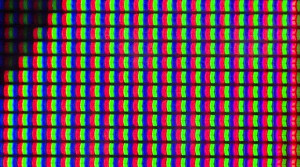
\includegraphics[scale=0.5]{Images/pixel.jpg}
 
 
 Maintenant que nous avons expliqué le principe du système RGB, nous allons expliquer son application sur une image. Etant donné la nature du système RGB, celui ci est donc représenté par la superposition de trois valeurs comprises entre 0 et 255, où une valeur représente la teinte associée à ça couleur primaire, l'image couleur est donc informatiquement une superposition de trois matrices. L'image ci-joint représente bien les possibilités que l'on peut obtenir en superposant les couleurs (si toutes les valeurs sont nulles on obtient du noir, si toutes les valeurs sont 255 on obtient du blanc etc...).
 
 
 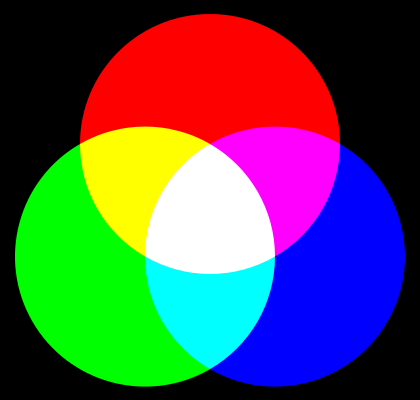
\includegraphics[scale=0.5]{Images/RGB.png}
 
 
 Malgrès le changement dû au passage à la couleur le principe des algorithmes que nous avons programmé reste le même, sauf que celui ci est appliqué aux trois matrices des couleurs primaires.\newline
 
 
 Un autre système, que l'on aurait pu utiliser est le système HSL (Hue Saturation Lightness ou Teinte Saturaion lumière), ce système est plus éloigné de la machine, mais plus près de la perception de l'homme. En effet, l'œil ne perçoit pas la couleur comme une superposition de couleurs, mais comme une sensation de luminosité. La saturation représente "l'intensité" de la couleur (si la couleur est plus ou moins forte), la teinte représente les différentes couleurs possibles dûes aux mélanges de couleurs primaires et enfin la lumière est remarquable selon si une image est plus ou moins sombre (proche du blanc ou du noir). La teinte est représentée par une valeur modulo 360, la saturation est une valeur entre 0 (sensation peu coloré) et 1 (sensation très coloré) et la lumisosité est une valeur entre 0 et 1 représentant le pourcentage de luminosité.


 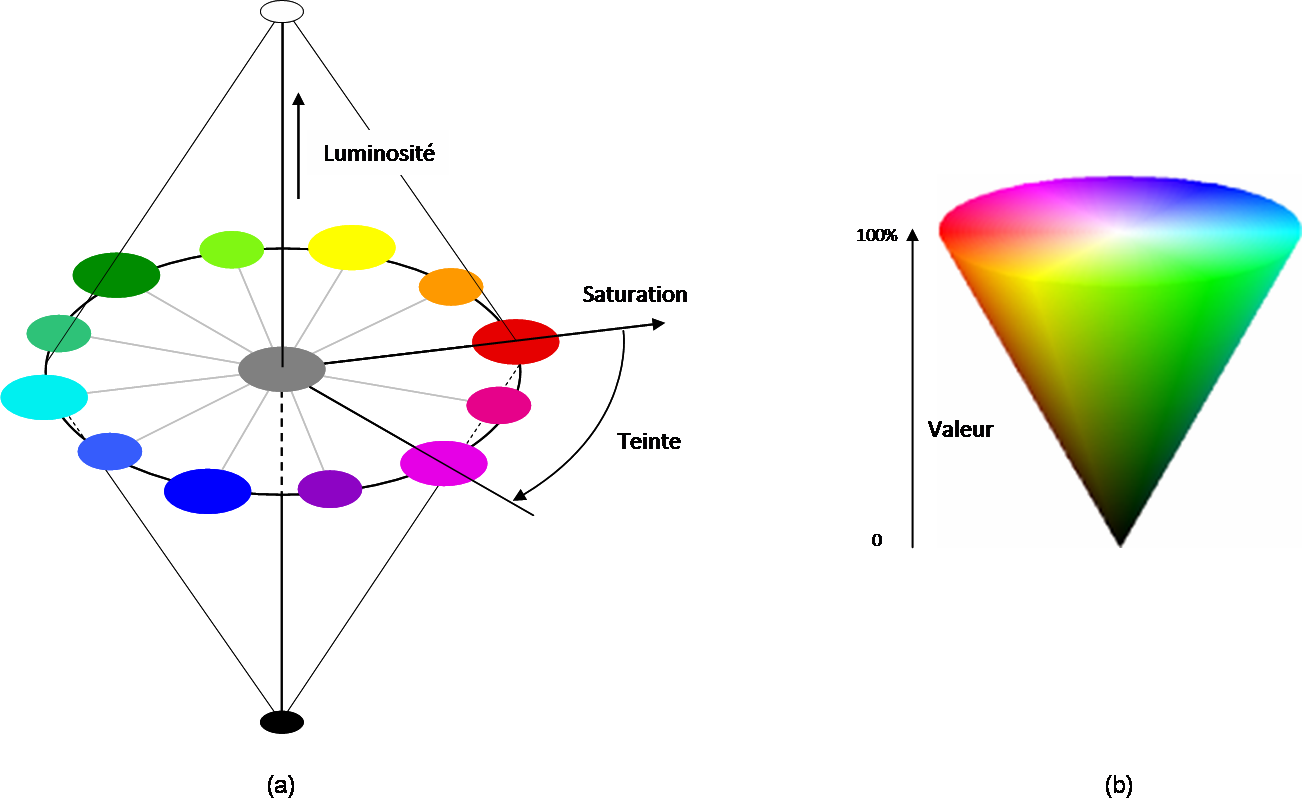
\includegraphics[scale=0.5]{Images/TSL.png}
 
 Il y a une grosse différence entre le nombre de couleurs que peux percevoir l'homme et le nombre de couleurs qui existent, en effet l'œil ne peut percevoir que jusqu'à un demi millions de couleurs différentes, alors que, par exemple le système RGB peut fournir 255 puissance 3 couleurs (soit environs 16 millions), il y a donc beaucoup de couleurs qui selon la machine sont différentes mais que l'homme ne peut différentiées.
